\documentclass{article}
\usepackage[utf8]{inputenc}
\usepackage[russian]{babel}
\usepackage[left=2cm,right=2cm,
top=2cm,bottom=2cm,bindingoffset=0cm]{geometry}
\usepackage{graphicx}
\usepackage{amsmath}
\usepackage{float}
\usepackage{listings}
\usepackage{url,textcomp}
\date{2019 г.}
\author{Кондратенко Федор, гр 13632/1}
\setlength{\parindent}{0pt}
\setlength{\parskip}{5pt plus 2pt minus 1pt}
\frenchspacing
\title{Отчет по заданию №4.1}
\begin{document}
	\maketitle
	\section*{Моделирование колебания одного груза}
	\paragraph*{Модель\\}
	За основу была взята модель Simscape, в которую был внесен ряд изменений, а именно: добавлена внешняя сила, изменен выходной сигнал модели -- вместо скорости выводится координата.
	\begin{figure}[H]
		\centering
		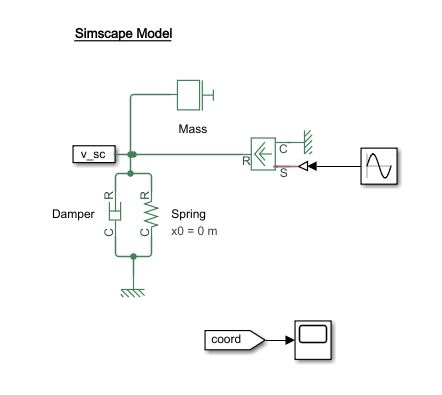
\includegraphics[width=0.7\linewidth]{sx_1_mod}
		\caption{Simscape модель}
		\label{fig:sx1mod}
	\end{figure}
	\begin{figure}[H]
		\centering
		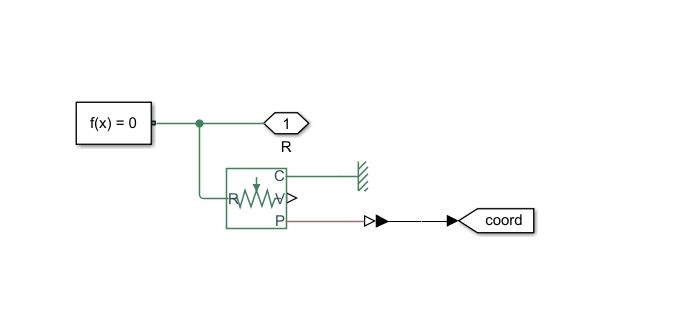
\includegraphics[width=0.7\linewidth]{sx_1_bs}
		\caption{Подсистема модели. Внесено изменение -- выводится координата вместо скорости.}
		\label{fig:sx1bs}
	\end{figure}
	Также было выполнено моделирование вынужденных колебаний при нулевых начальных условиях на частоте резонанса:
	\begin{figure}[H]
		\centering
		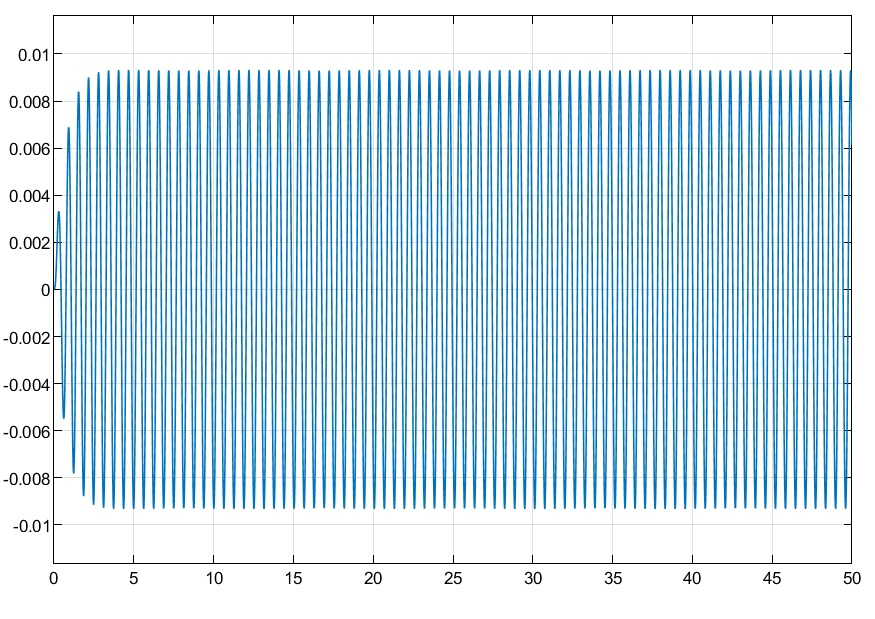
\includegraphics[width=0.7\linewidth]{graph1}
		\caption{Вынужденные колебания груза на пружине при нулевых начальных условиях на частоте резонанса $\omega = 10.5$}
		\label{fig:graph1}
	\end{figure}
	\section*{Моделирование колебаний двух последовательно соединенных грузов}
	За основу была взята модель Simscape, в которую были внесены изменения: добавлены внешние силы, изменен выходной сигнал модели -- вместо скорости выводится координата.
	\begin{figure}[H]
		\centering
		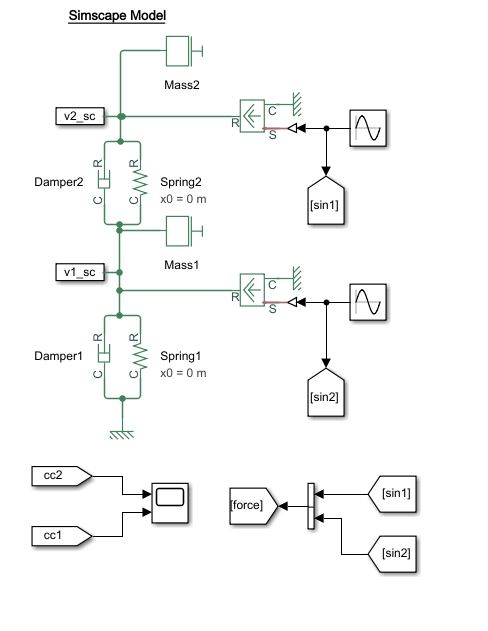
\includegraphics[width=0.7\linewidth]{sx_2}
		\caption{Блок-схема модели}
		\label{fig:sx2}
	\end{figure}
	Помимо этого, уравнение колебаний двух масс было приведено к матричному виду. Блок-схема матричного уравнения:
	\begin{figure}[H]
		\centering
		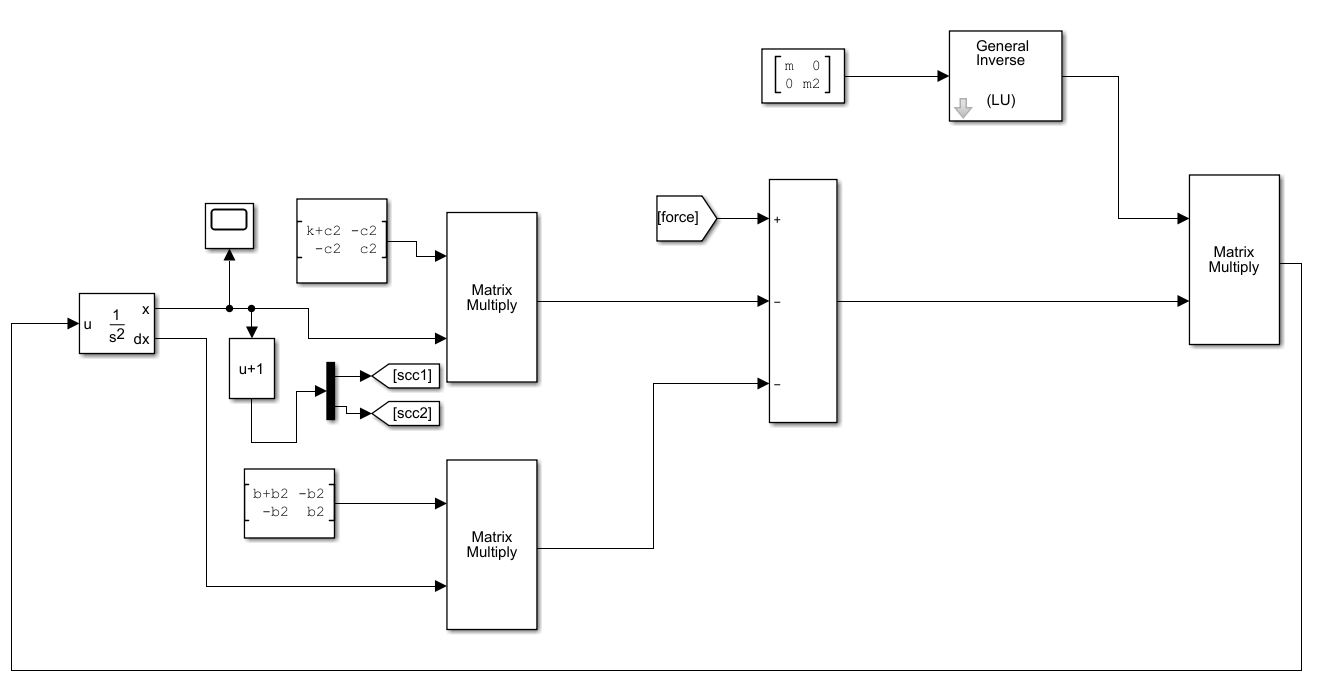
\includegraphics[width=1\linewidth]{matr_sx}
		\caption{Блок-схема матричного уравнения. Параметры нижней массы были взяты из примера, параметры верхней массы -- из предыдущего задания: $m_2 = 30,\ b_2 = 1200,\ c_2 = 4650$.}
		\label{fig:matrsx}
	\end{figure}
	Для модели были определены собственные частоты как аналитическим, так и графическим методом.\\
	Данные, полученные аналитически: $k_1 = 3.336,\ k_2 = 39.33$\\
	Для того, чтобы определить собственные частоты графически с помощью линейного анализа, понадобилось уменьшить коэффициент $b_2$:
	\begin{figure}[H]
		\centering
		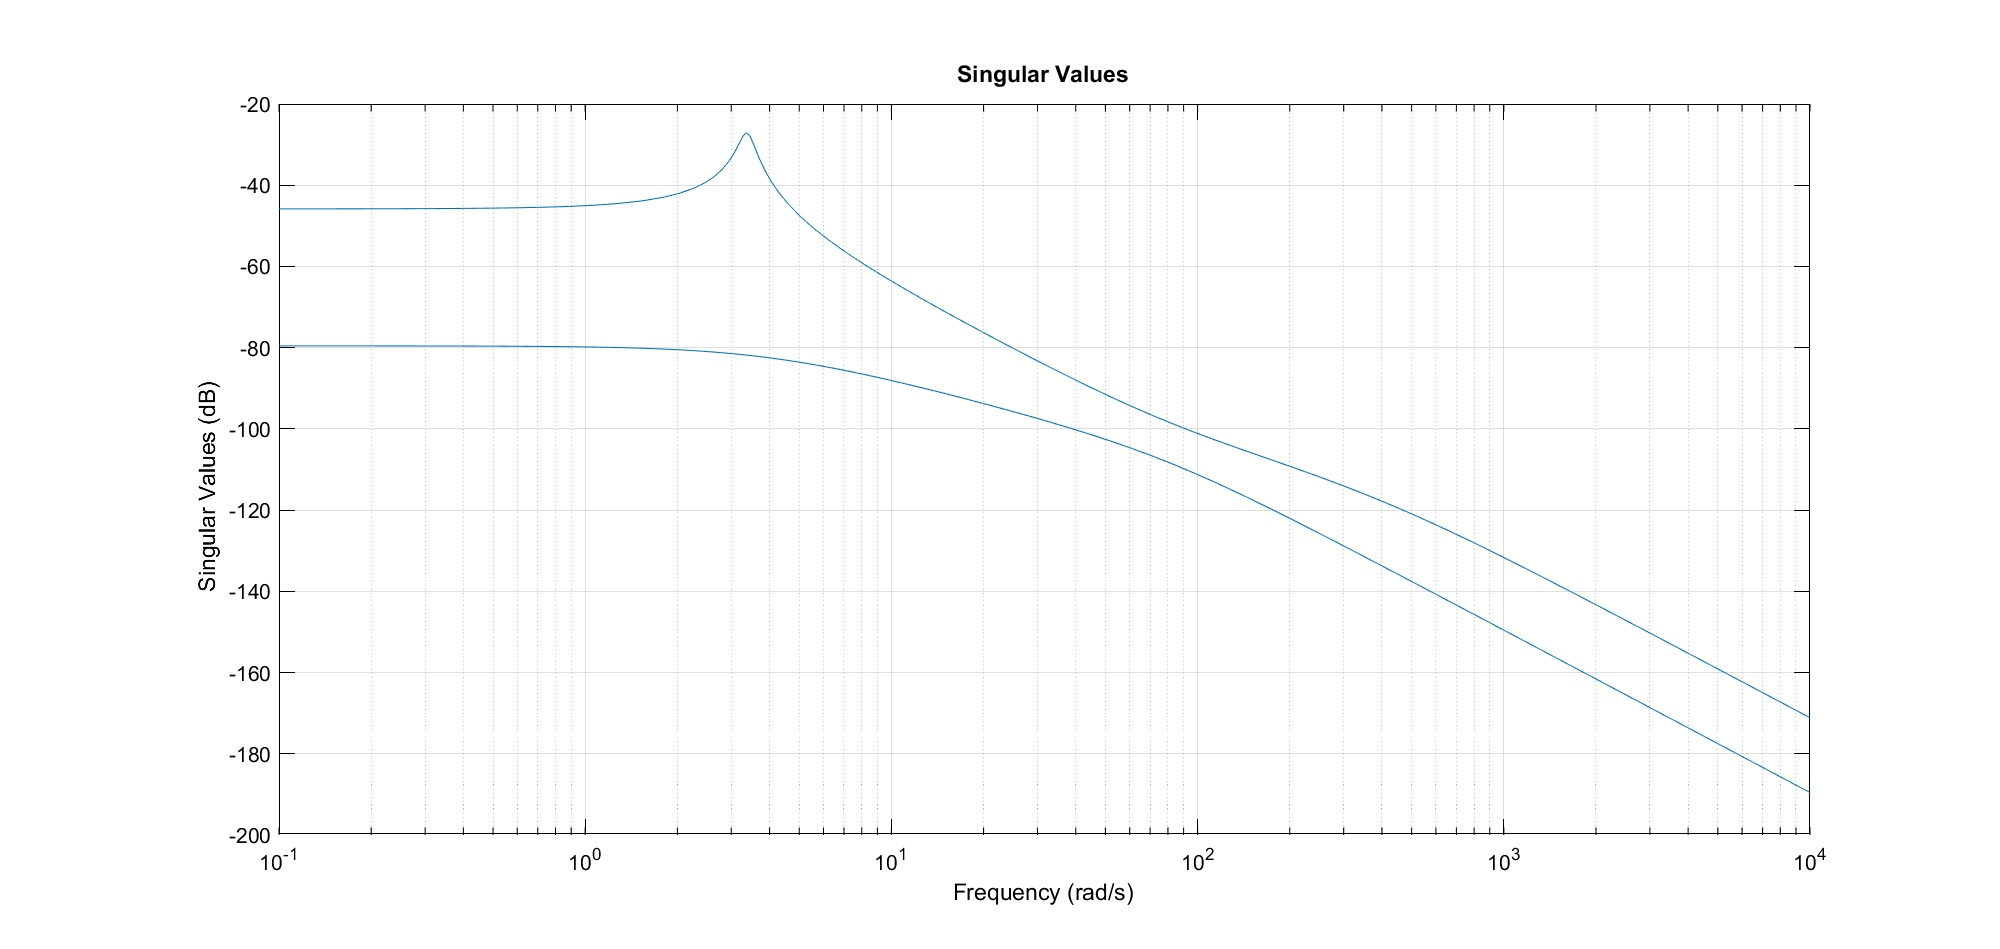
\includegraphics[width=1\linewidth]{sv_b1200}
		\caption{$b = 1200$, второй резонанс не обнаруживается}
		\label{fig:svb1200}
	\end{figure}
	\begin{figure}[H]
		\centering
		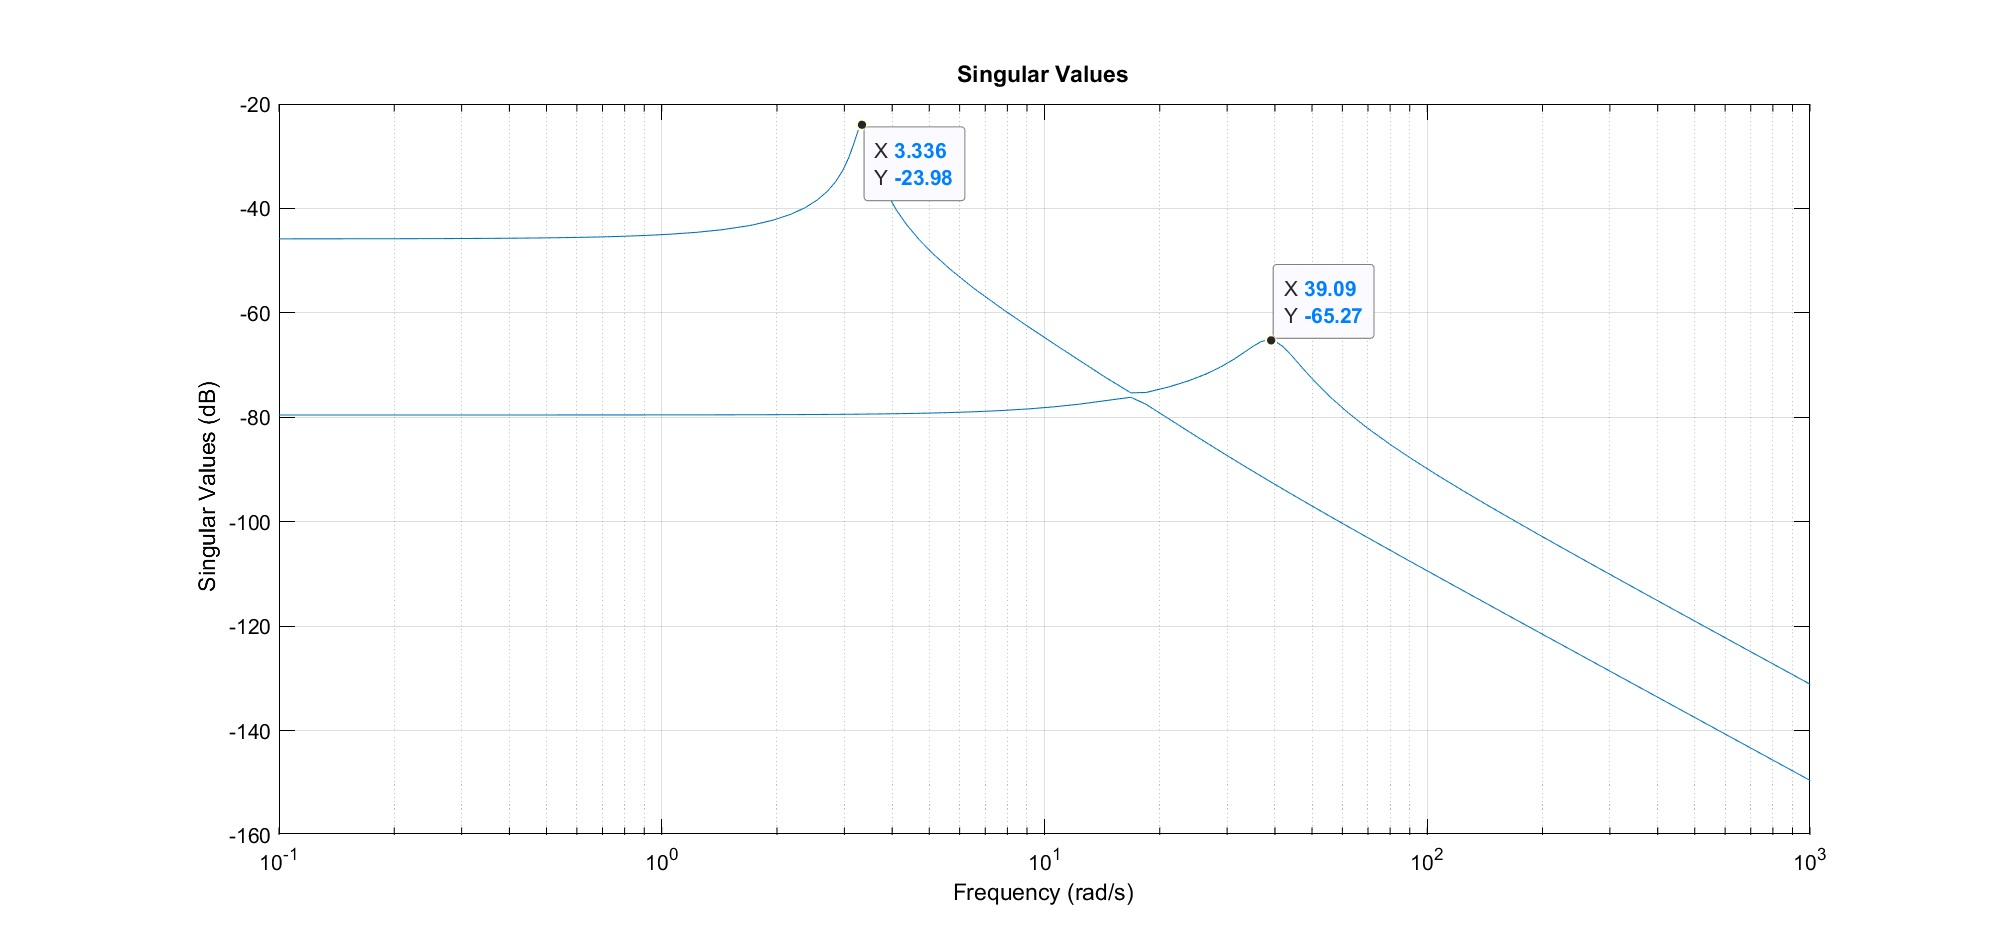
\includegraphics[width=1\linewidth]{sv_b30}
		\caption{$b=30$, оба резонанса отчетливо видны}
		\label{fig:svb30}
	\end{figure}
	По данным линейного анализа: $k_1 = 3.336,\ k_2 = 39.09$\\
	Результаты моделирования выводились на один осциллограф:
	\begin{figure}[H]
		\centering
		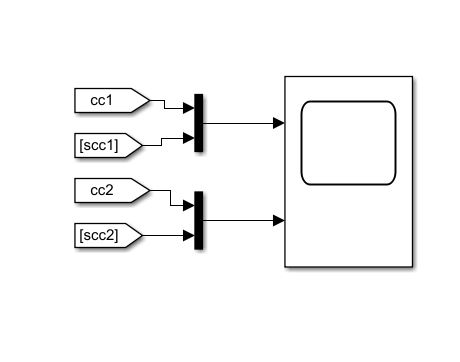
\includegraphics[width=0.7\linewidth]{out}
		\caption{Вывод данных}
		\label{fig:out}
	\end{figure}
	
	\paragraph*{Результаты моделирования\\}
	Моделирование свободных колебаний:
	\begin{figure}[H]
		\centering
		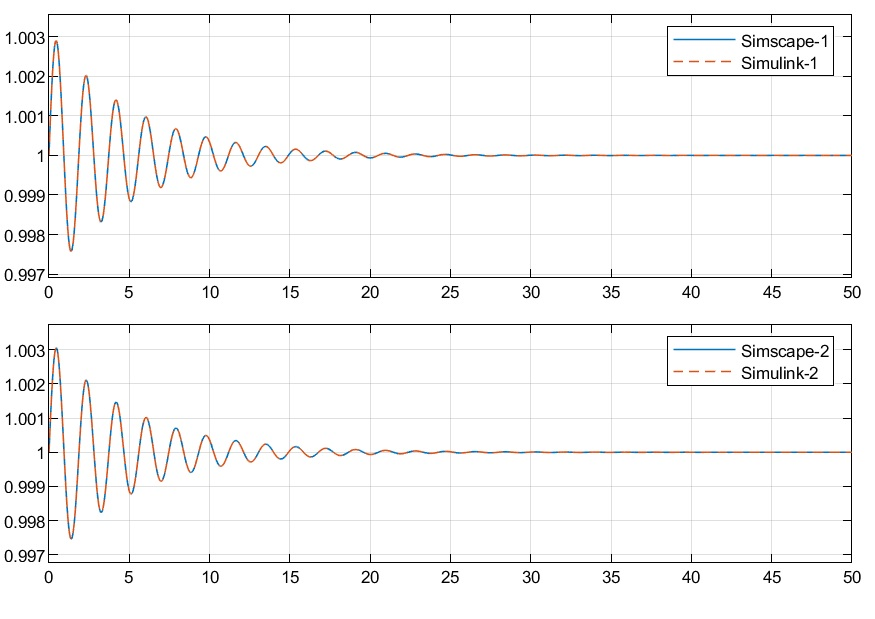
\includegraphics[width=0.7\linewidth]{v001002}
		\caption{Моделирование свободных колебаний при учете трения, $v_1 = 0.01,\ v_2 = 0.02,\ b_1 = 10,\ b_2 = 1200$}
		\label{fig:v0}
	\end{figure}
	\begin{figure}[H]
		\centering
		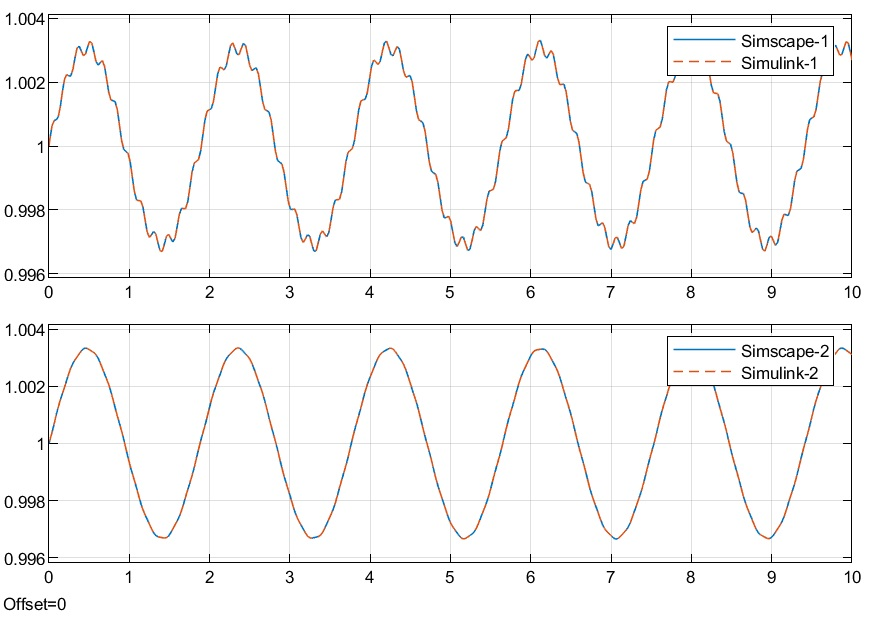
\includegraphics[width=0.7\linewidth]{b=0}
		\caption{Моделирование свободных колебаний без трения, $b_1 = b_2 = 0$, остальные параметры не менялись.}
		\label{fig:b0}
	\end{figure}
	Отчетливо виден бигармонический процесс.\\
	Моделирование вынужденных колебаний:
	\begin{figure}[H]
		\centering
		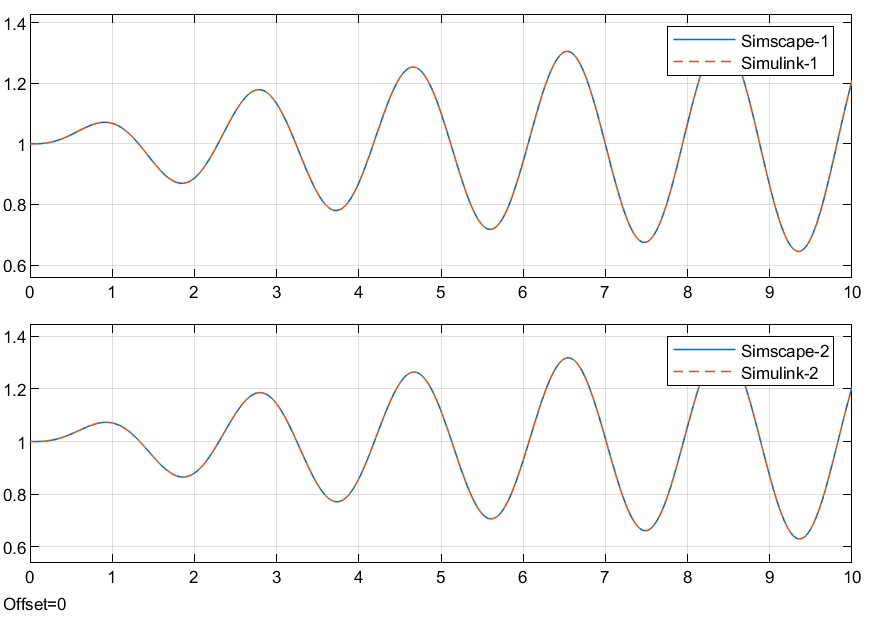
\includegraphics[width=0.7\linewidth]{nizr1}
		\caption{Сила на частоте первого резонанса приложена к нижнему грузу}
		\label{fig:nizr1}
	\end{figure}
	\begin{figure}[H]
		\centering
		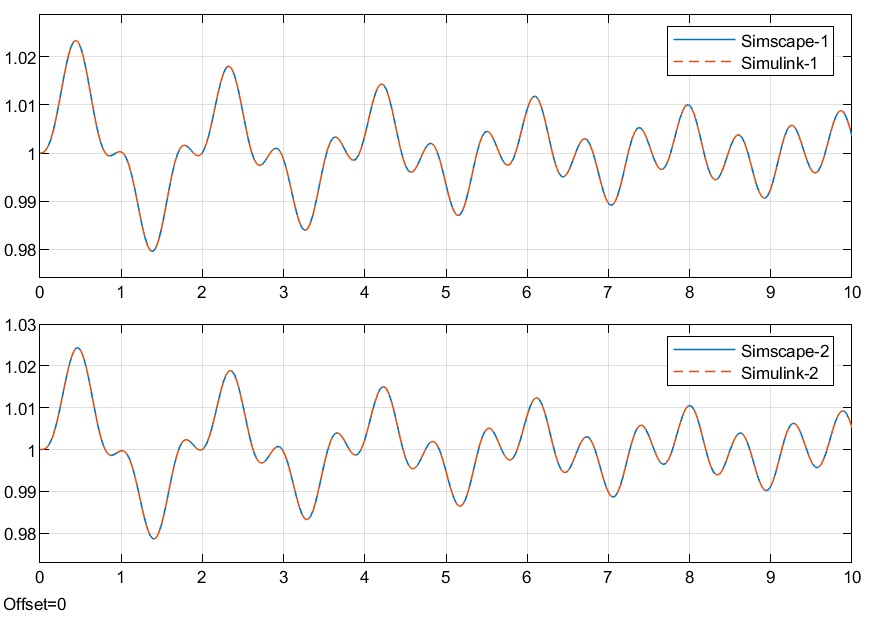
\includegraphics[width=0.7\linewidth]{nizr1r2}
		\caption{Сила на частоте $\omega = 10$ между двумя резонансами приложена к нижнему грузу}
		\label{fig:nizr1r2}
	\end{figure}
	\begin{figure}[H]
		\centering
		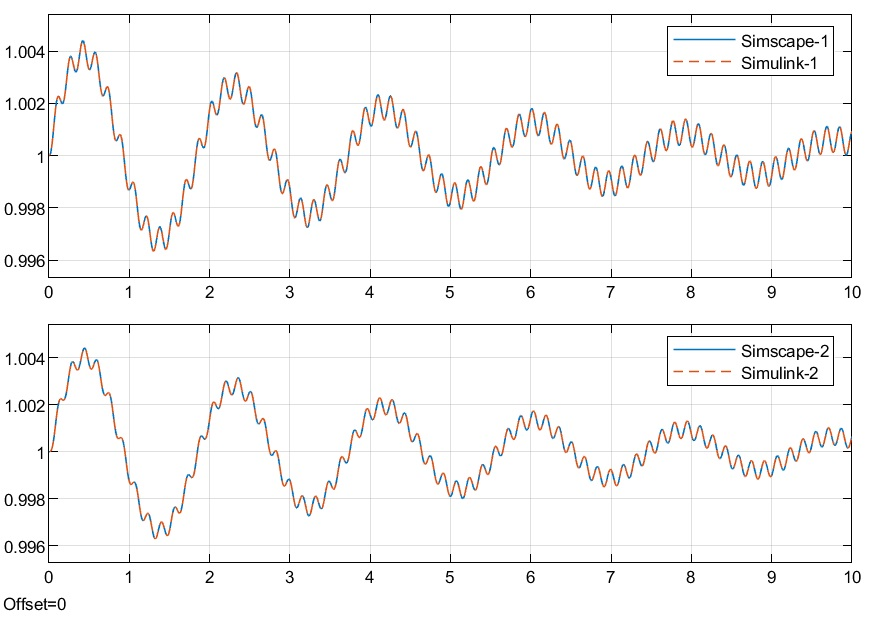
\includegraphics[width=0.7\linewidth]{nizr2}
		\caption{Сила на частоте второго резонанса приложена к нижнему грузу}
		\label{fig:nizr2}
	\end{figure}
	\begin{figure}[H]
		\centering
		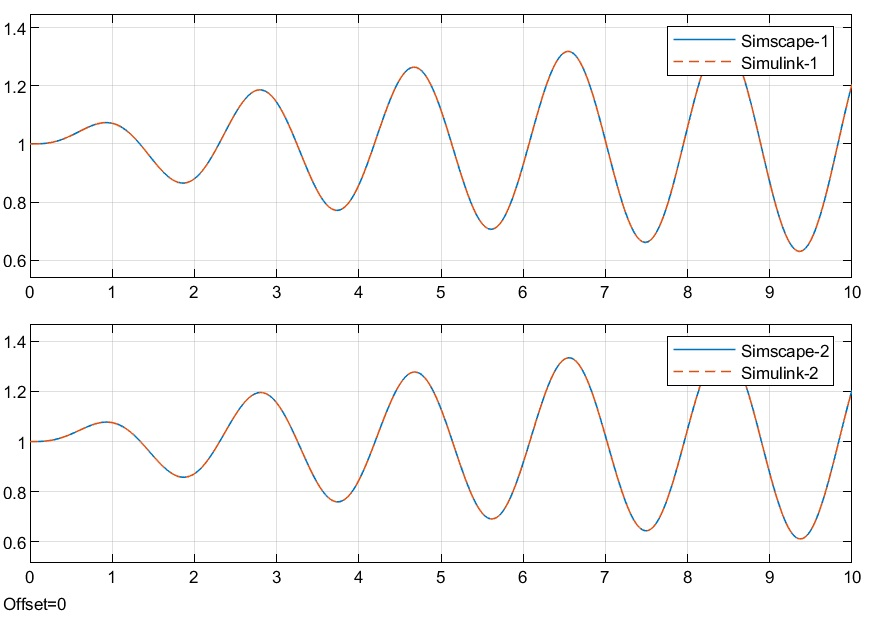
\includegraphics[width=0.7\linewidth]{verxr1}
		\caption{Сила на частоте первого резонанса приложена к верхнему грузу}
		\label{fig:verxr1}
	\end{figure}
	\begin{figure}
		\centering
		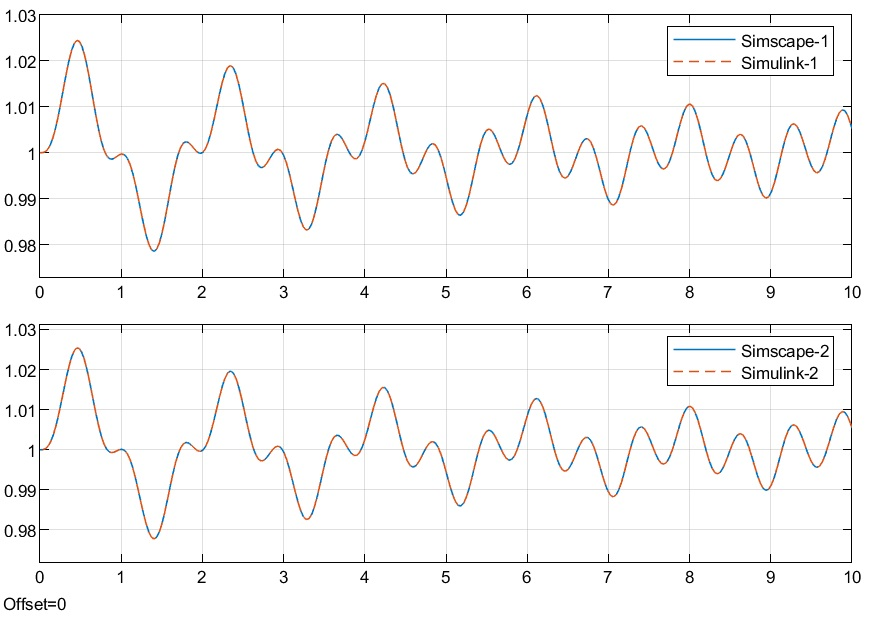
\includegraphics[width=0.7\linewidth]{verx10}
		\caption{Сила на частоте $\omega = 10$ между двумя резонансами приложена к верхнему грузу}
		\label{fig:verx10}
	\end{figure}
	\begin{figure}[H]
		\centering
		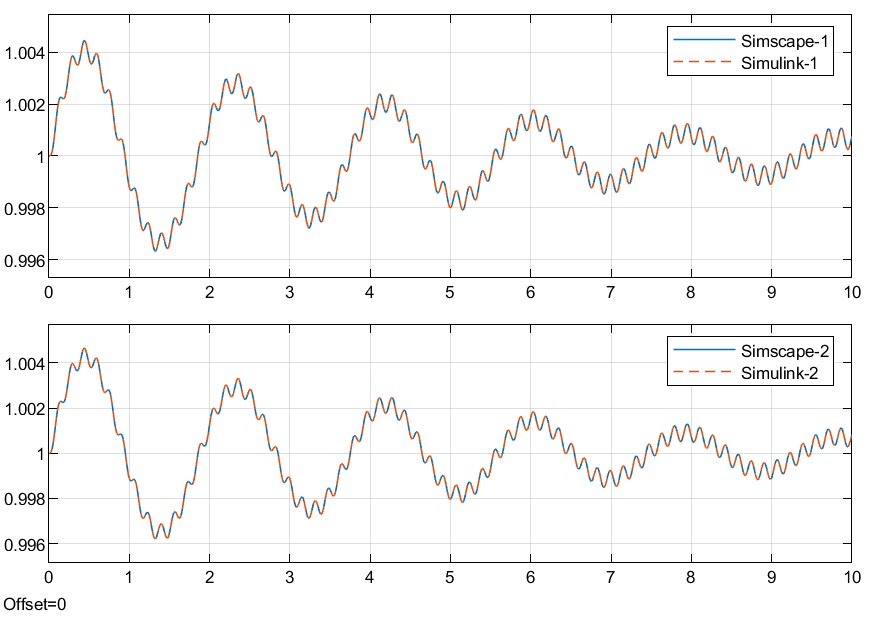
\includegraphics[width=0.7\linewidth]{verxr2}
		\caption{Сила на частоте второго резонанса приложена к верхнему грузу}
		\label{fig:verxr2}
	\end{figure}
	Можно заметить сходство между графиками колебаний при приложении силы как ко второму, так и к первому грузу.
	\begin{figure}[H]
		\centering
		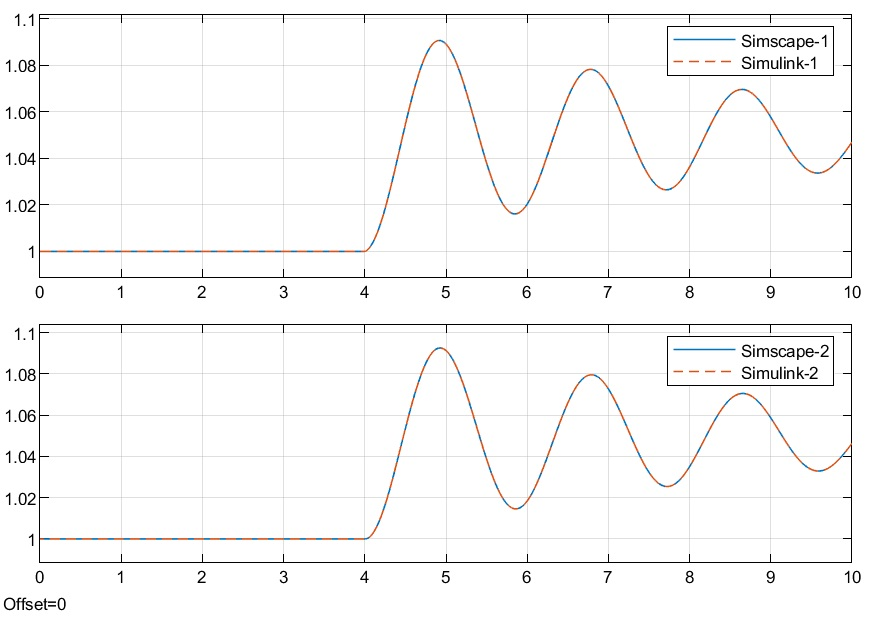
\includegraphics[width=0.7\linewidth]{step}
		\caption{Реакция системы на Step-сигнал}
		\label{fig:step}
	\end{figure}
	Из графика следует, что происходят затухающие колебания. После их окончания под действием постоянной силы система останется в неустойчивом состоянии -- пружины будут растянуты, и как только действие постоянной силы исчезнут, возникнут свободные колебания.
\end{document}